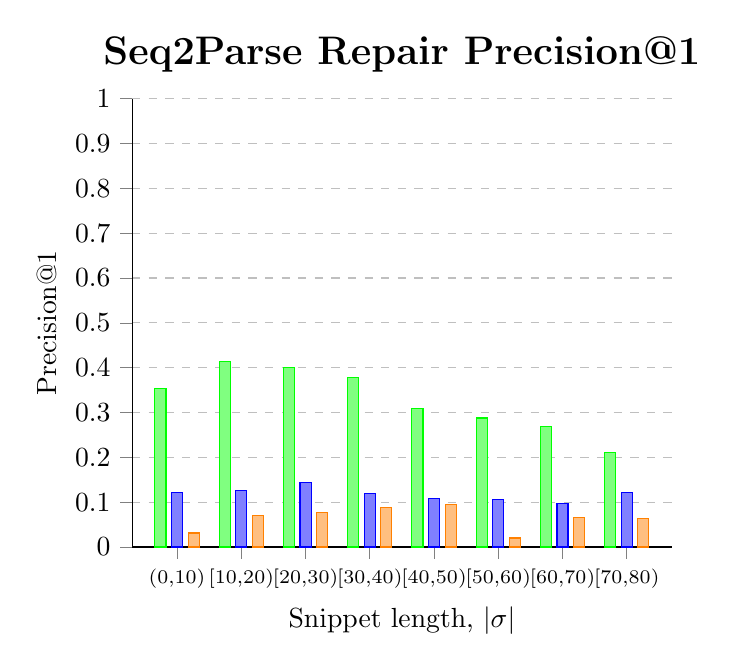
\begin{tikzpicture}
  \begin{axis}[
    xlabel={Snippet length, $|\sigma|$},
    ylabel={Precision@1},
    title={\Large\textbf{Seq2Parse Repair Precision@1}},
    ybar,
    axis lines*=left,
    xtick={0, 10, 20, 30, 40, 50, 60, 70},
    ytick={0, 0.1, 0.2, 0.3, 0.4, 0.5, 0.6, 0.7, 0.8, 0.9, 1.0},
    xticklabels={{(}0{,}10{)}, {[}10{,}20{)}, {[}20{,}30{)}, {[}30{,}40{)}, {[}40{,}50{)}, {[}50{,}60{)}, {[}60{,}70{)}, {[}70{,}80{)}},
    x tick label style={font=\scriptsize},
    ymax=1.0,
    ymin=0.0,
    bar width=4pt,
    ymajorgrids=true,
    grid style=dashed,
    tick align=outside,
    tick pos=left,
  ]

  \addplot[green, fill=green!50] coordinates {(0, 0.352631) (10, 0.413115) (20, 0.400502) (30, 0.378440) (40, 0.308869) (50, 0.287755) (60, 0.268817) (70, 0.210526)};
  \addplot[blue, fill=blue!50] coordinates {(0, 0.122529) (10, 0.126453) (20, 0.144192) (30, 0.118483) (40, 0.108007) (50, 0.106849) (60, 0.097403) (70, 0.122047)};
  \addplot[orange, fill=orange!50] coordinates {(0, 0.03125) (10, 0.070922) (20, 0.077348) (30, 0.087629) (40, 0.094675) (50, 0.02) (60, 0.066038) (70, 0.063291)};

  \end{axis}
\end{tikzpicture}